% Alternative Fig. 1 (teaser): qualitative examples on the left, the plot on the right.
% Build:  cd figures/src && tectonic fig1_qual.tex && mv fig1_qual.pdf ../teaser_qual.pdf
% Examples live in teaser_qual_examples.tex. teaser_qual_plot.pdf is the plot cropped, as
% vector, from ../teaser.pdf. Row colors are those of drawio_files/teaser.drawio.
\documentclass[tikz,border={0.5pt 0.5pt 0.5pt 2pt}]{standalone}
\usepackage{fontspec}
\setmainfont{texgyretermes}[Extension=.otf,UprightFont=*-regular,BoldFont=*-bold,
  ItalicFont=*-italic,BoldItalicFont=*-bolditalic]
\usepackage{xcolor}
\usetikzlibrary{calc}

\definecolor{ink}{HTML}{000000}
\definecolor{bad}{HTML}{DC5B52}
\definecolor{good}{HTML}{1D8159}
\definecolor{ours}{HTML}{3775BA}
\definecolor{base}{HTML}{767676}
\definecolor{rowA}{HTML}{EEEEEE}\definecolor{rowAl}{HTML}{36393D}
\definecolor{rowB}{HTML}{F8E4E4}\definecolor{rowBl}{HTML}{B85450}
\definecolor{rowC}{HTML}{DDEEFF}\definecolor{rowCl}{HTML}{66B2FF}

\newcommand{\fs}[1]{\fontsize{#1pt}{\dimexpr #1pt*118/100\relax}\selectfont}
\newcommand{\ok}{\tikz[baseline=-0.55ex]{\fill[good](0,0) circle(2.7pt);
  \draw[white,sharp corners,line width=0.6pt,line cap=round,line join=round]
  (-1.35pt,0.05pt)--(-0.45pt,-0.85pt)--(1.35pt,0.95pt);}}
\newcommand{\no}{\tikz[baseline=-0.55ex]{\fill[bad](0,0) circle(2.7pt);
  \draw[white,sharp corners,line width=0.6pt,line cap=round]
  (-0.95pt,-0.95pt)--(0.95pt,0.95pt)(-0.95pt,0.95pt)--(0.95pt,-0.95pt);}}
% Content of the qualitative teaser (fig1_qual.tex). Every string must be a real model output.
% Fill from select_teaser_examples.py (Qwen3-VL-4B, base vs. full GRPO, LATCH at tau_p = 2).
% Photos are looked up in this folder; a missing one renders as a dashed "photo needed" box.

% ---- Robustness: corrupted, answerable; base wrong, GRPO right, LATCH does not fire.
% TODO: no such example exists outside outputs/ on the cluster. After filling in, set the marks
% to \no, \ok, \ok.
\def\RobImg{qual_robust.jpg}
\def\RobQ{TODO: question}
\def\RobBase{TODO}   \def\RobBaseMark{}
\def\RobFT{TODO}     \def\RobFTMark{}
\def\RobOurs{TODO}   \def\RobOursMark{}

% ---- Abstention: unanswerable VizWiz question.
% Verbatim from Fig. supp_qual_vizwiz (suppl.tex): "What is this package?", GRPO probe logit
% 3.86 > tau = 2. The photo is figures/supp_qual/vz_package.jpg on the cluster.
\def\AbsImg{vz_package.jpg}
\def\AbsQ{``What is this package?''}
\def\AbsBase{Unanswerable}   \def\AbsBaseMark{\ok}
\def\AbsFT{Book}             \def\AbsFTMark{\no}
\def\AbsOurs{Unanswerable}   \def\AbsOursMark{\ok}


\begin{document}
\begin{tikzpicture}[x=1pt,y=1pt,
  every node/.style={inner sep=0pt, outer sep=0pt, text=ink},
  chip/.style={draw=ink, line width=0.6pt, rounded corners=2pt, fill=white, font=\fs{7.4},
               minimum height=13pt, minimum width=84pt, inner xsep=3pt},
  coltitle/.style={font=\fs{8}\bfseries, anchor=south},
  colsub/.style={font=\fs{6.8}\itshape, anchor=north},
  question/.style={font=\fs{6.8}\itshape, align=center, text width=90pt, anchor=north},
]
\def\XR{108}\def\XA{204}   % column centres
\def\IW{64}\def\IH{46}     % photo slot
% photo or a visible placeholder: \photo{file}{centre x}
\newcommand{\photo}[2]{%
  \IfFileExists{#1}{\node[anchor=north] at (#2,-20)
    {\includegraphics[width=\IW pt,height=\IH pt,keepaspectratio]{#1}};}{%
    \draw[bad, line width=0.6pt, dash pattern=on 2pt off 1.5pt]
      (#2-\IW/2,-20) rectangle (#2+\IW/2,-20-\IH);
    \node[font=\fs{6.4}, text=bad] at (#2,-20-\IH/2) {photo needed};}}
% \row{y}{fill}{line}{label}{label color}{rob}{rob mark}{abs}{abs mark}
\newcommand{\row}[9]{%
  \draw[#3, line width=0.6pt, fill=#2, rounded corners=3pt] (0,#1-11.5) rectangle (252,#1+11.5);
  \node[font=\fs{7.4}\bfseries, align=left, text=#5, anchor=west] at (5,#1) {#4};
  \node[chip] at (\XR,#1) {};
  \node[font=\fs{7.4}, anchor=west] at (\XR-39,#1) {#6};
  \node at (\XR+35,#1) {#7};
  \node[chip] at (\XA,#1) {};
  \node[font=\fs{7.4}, anchor=west] at (\XA-39,#1) {#8};
  \node at (\XA+35,#1) {#9};
}
% ---------------------------------------------------------------- column heads
\node[coltitle] at (\XR,-9) {Robustness};
\node[colsub] at (\XR,-10) {corrupted, answerable};
\node[coltitle] at (\XA,-9) {Abstention};
\node[colsub] at (\XA,-10) {unanswerable};
\photo{\RobImg}{\XR}
\photo{\AbsImg}{\XA}
\node[question] at (\XR,-68.5) {\RobQ};
\node[question] at (\XA,-68.5) {\AbsQ};
% ---------------------------------------------------------------- rows
\row{-92}{rowA}{rowAl}{Base VLM}{base}{\RobBase}{\RobBaseMark}{\AbsBase}{\AbsBaseMark}
\row{-118}{rowB}{rowBl}{Robust\\[-1pt]fine-tuned}{bad}{\RobFT}{\RobFTMark}{\AbsFT}{\AbsFTMark}
\row{-144}{rowC}{rowCl}{+ LATCH\\[-1pt](ours)}{ours}{\RobOurs}{\RobOursMark}{\AbsOurs}{\AbsOursMark}
% ---------------------------------------------------------------- plot (unchanged)
\node[anchor=east] at (486,-78) {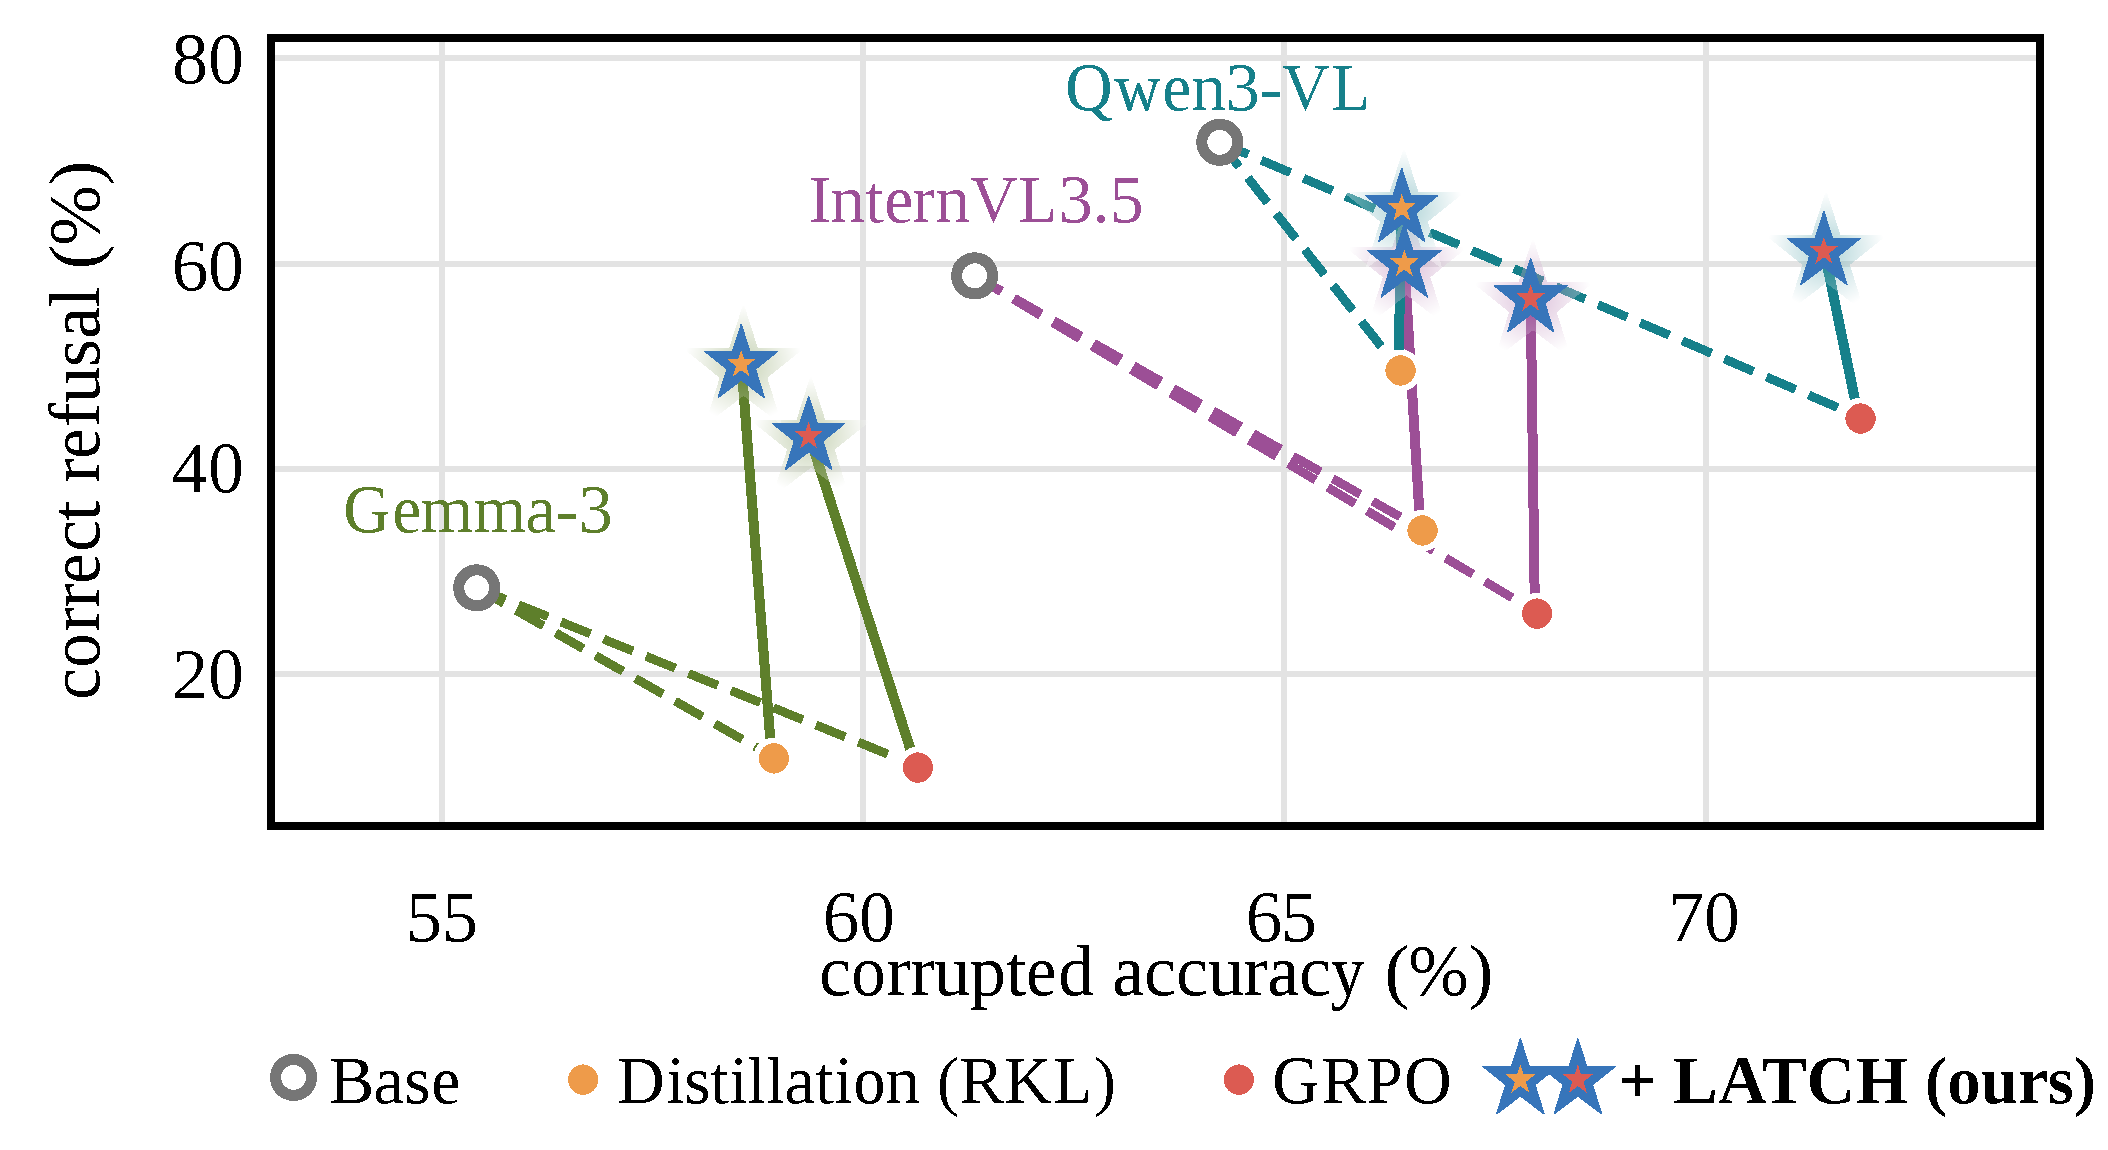
\includegraphics[width=224pt]{teaser_qual_plot.pdf}};
\end{tikzpicture}
\end{document}
